\documentclass{article}
\usepackage[margin=1.25in]{geometry}
\usepackage{graphicx}
\usepackage{physics}

\title{Photon Pairs Exhibit Polarization Correlations Characteristic of Quantum Entanglement}
\author{Luke Burns}
\date{13 March 2016}

\begin{document}

\maketitle

\begin{abstract}
  Linearly polarized photons produced by a 407~nm pump laser undergo Type-I Spontaneous Parametric Down Conversion (SPDC), facilitated by two Beta Barium Borate (BBO) crystals, yielding pairs of entangled 814~nm photons with correlated polarizations. These photons pass through polarizers, and coincidences are counted for varied polarization configurations. The number of coincidences determined for characteristic polarization configurations (+45, +45) and (+45, -45) differ from what are predicted classically.
\end{abstract}

\section{Introduction}

Quantum entanglement is a hallmark of quantum mechanics. Einstein brought the phenomenon to universal awareness in 1935, when he proposed the experiment as a demonstration of a paradox.\cite{einstein} He argued that the experiment violated the basic physical principle of locality, which says that physical objects are only influenced by their immediate surroundings, at least not without some medium facilitating the interaction. It is a principle central in our human experience. Einstein reasoned that quantum mechanics must be incomplete and missing a description of some underlying hidden variables.

In 1964, John Stewart Bell drew up a set of inequalities that local hidden variable theories must obey. The local hidden variable theories obeying these inequalities rested upon two principles: locality and realism, which was also assumed by Einstein. The principle of realism says that properties of a system exist independently of their observation. If these inequalities are demonstrably violated, then physicists would be forced to abandon at least one of these principles.\cite{bell}

In 1966, Bell proved the Bell-Kochen-Specker theorem, which elaborated upon the issue of realism, showing that there is a contradiction between thinking that hidden properties corresponding to observables have definite values at any given time and the values of those properties are independent of the device used to measure them.\cite{bell2}

The Copenhagen interpretation opts to abandon both locality and realism, but there do exist interpretations of quantum mechanics which opt to preserve locality and abandon realism, or vice versa, and remain consistent in all predictions. An example of the former kind of theory is Relational Quantum Mechanics (RQM), in which the properties of a system exist only in reference to another system, i.e. relationally.\cite{rovelli}

In the early 1980s, Alain Aspect performed experiments using entangled photons and confirmed statistics which violated Bell's inequalities, hence definitively eliminating a local and real picture of nature.\cite{aspect} Since then, many inequalities have been proposed and loopholes tested, and experiments continue to validate quantum mechanics.

In this experiment, photons are downconverted into pairs of polarization correlated photons via Spontaneous Parametric Downconversion (SPDC), which are passed through polarizers and detected for coincidences for various polarizer angle configurations. We show that classical predictions for coincidence probabilities theoretically contradict quantum predictions. This experiment invalidates the classical model.

\section{Theory}

\subsection{Downconversion}

SPDC is a process in which one photon is converted into two photons each with half the energy, via the nonlinearity of a material. In Type-I SPDC, downconverted photons are polarized in the same direction as each other but perpendicular to the incident photon.

Due to dispersion, downconverted photon pairs propagate at a different speed than the incident photon, disrupting phase coherence of incidence and downconverted photons and reducing the efficiency of the conversion process. Only a small fraction of incident photons undergo SPDC. 

This problem can be resolved by use of birefringent materials, in which the refractive index is dependent on polarization. Using birefringence, one can maximize the efficiency of the conversion process by satisfying the phase matching condition

\begin{equation}
  \frac{\sin^2{\theta}}{n_e(\omega)^2} + \frac{\cos^2{\theta}}{n_o(\omega)^2} = \frac{\sec^2{\alpha}}{n_o(\omega/2)^2}, \label{eq:dc}
\end{equation}

where $2 \alpha$ is the angle between downconverted photons, $\theta$ is the angle the incident photon makes with the crystal's optic axis, $n_e$ and $n_0$ are the wavelength-dependent refractive indices for the BBO.

In this experiment, a pair of Beta Barium Borate (BBO) crystals with cut $\theta=30^{\circ}$ facilitate Type-I SPDC of mostly vertically polarized, 407~nm photons. With this cut and energy, the angle at which the downconverted photons propagate through the crystal is $\alpha = 3.2^{\circ}$. Each propagates at the angle $\alpha$ relative to the direction of the incident photon, because the two downconverted photons have the same energy, half that of the incident photon (i.e. twice the wavelength, 814~nm).

Additionally, incident photons are polarized at $45^{\circ}$ so that downconverted photons are produced with $0^{\circ}$ (horizontal) and $90^{\circ}$ (vertical) polarizations with equal probability.

\subsection{Classical Correlations}

Malus' law governs the effect of perfect polarizers on light passing through and is given by

\begin{equation}
  I = I_0 \cos^2{\theta},
\end{equation}

where $\theta = \theta_1 - \theta_0$ and $I_0$ are depicted in Figure \ref{fig:malus}.

\begin{figure}[!h]
  \centering
  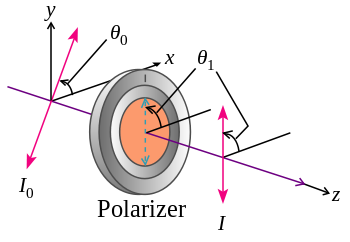
\includegraphics[width=0.5\textwidth]{malus}
  \caption{Light passing through linear polarizer as described by Malus' Law. Here $\theta = \theta_1 - \theta_0$. \label{fig:malus}}
\end{figure}

The counting of photons is achieved by use of a photomultiplier tube which exploits the photoelectric effect, in which the intensity of incident light is proportional to the number of photon counts. 

As an example, if a pair of photons is produced, traveling along paths $p$ and $p'$, and the corresponding polarizer filters along each path are configured to $\theta_1 = 45^{\circ}$ and $\theta_1' = -45^{\circ}$, then Malus' Law implies that the intensity of incident horizontally or vertically polarized light passed through each filter is reduced by half. Hence, the number of individual counts through each polarizer is halved, and the total number of coincidences is quartered. Coincidence probabilities for a variety of polarizer configurations are shown in Table \ref{tab:classical}.

\begin{table}[!h]
  \centering
  \begin{tabular}{ c c }
    Polarizer Angles & Probability of Coincidence \\ \hline
    (0, 0) & 50\% \\
    (90, 90) & 50\% \\
    (45, 45) & 25\% \\
    (45, -45) & 25\% \\
    (0, 90) & 0\%
  \end{tabular}
  \caption{Classical prediction of coincidence probabilities for correlated photon pairs. \label{tab:classical}}
\end{table}

\subsection{Quantum Correlations}

A pair of downconverted photons exist in the state 

\begin{equation}
  \ket{\psi} = \cos(\theta) \ket{H}_1 \ket{H}_2 + e^{i\phi} \sin(\theta) \ket{V}_1 \ket{V}_2,
\end{equation}

given an incident photon polarized angle $\theta$ relative to vertical with a correction term $\phi$ due to a phase shift between vertical and horizontal polarization components, in addition to dispersion and birefringence in the BBO crystals.

With $\theta = 45^{\circ}$ and $\phi = 0$, the state is maximally entangled, and the pair of downconverted photons is described by the construction of Einstein, Podolsky, and Rosen:\cite{dehlinger}

\begin{equation}
  \ket{\psi_{\text{EPR}}} = \frac{1}{\sqrt{2}}(\ket{H}_1 \ket{H}_2 + \ket{V}_1 \ket{V}_2). \label{eq:epr}
\end{equation}

In the basis of the polarizer filters at angle $\gamma$, the  polarization of the photons are

\begin{equation}
  \ket{H_\gamma} = \cos(\gamma) \ket{H} + \sin(\gamma) \ket{V} \label{eq:h}
\end{equation}

and 

\begin{equation}
  \ket{V_\gamma} = \cos(\gamma) \ket{V} - \sin(\gamma) \ket{H}. \label{eq:v}
\end{equation}

The probability that photon 1 is detected at a polarizer angle $\alpha$ and photon 2 at a polarizer angle $\beta$ is given by

\begin{equation}
  P(\alpha, \beta) = |\bra{V_\alpha}_1\bra{V_\beta}_2 \ket{\psi_{\text{EPR}}}|^2 = \frac{1}{2} \cos^2(\beta-\alpha). \label{eq:quantum}
\end{equation}

For $\alpha = 45^{\circ}$ and $\beta = -45^{\circ}$, in stark contrast to the classical account, the coincidence probability $P(45^{\circ}, -45^{\circ}) = 0$. Coincidence probabilities for a range of polarizer configurations are shown in Table \ref{tab:quantum}.

\begin{table}[!h]
  \centering
  \begin{tabular}{ c c }
    Polarizer Angles & Probability of Coincidence \\ \hline
    (0, 0) & 50\% \\
    (90, 90) & 50\% \\
    (45, 45) & 50\% \\
    (45, -45) & 0\% \\
    (0, 90) & 0\%
  \end{tabular}
  \caption{Quantum prediction of coincidence probabilities for correlated photon pairs. \label{tab:quantum}}
\end{table}

A comparison of the classical and quantum models is shown in Table \ref{tab:vs}. The key differences between the models are the probabilities for the polarizer angle configurations (45, 45) and (-45, 45).

\begin{table}[!h]
  \centering
  \begin{tabular}{ c c c }
    Polarizer Angles & Classical Probability & Quantum Probability \\ \hline
    (0, 0)     & 50\% & 50\% \\
    (90, 90)   & 50\% & 50\% \\
    (+45, +45) & 25\% & 50\% \\
    (-45, +45) & 25\% &  0\% \\
    (0, 90)    &  0\% &  0\%
  \end{tabular}
  \caption{Key differences between classical and quantum models are in the (+45, +45) and (-45, +45) configurations. \label{tab:vs}}
\end{table}

\section{Experimental Procedure}

Figure \ref{fig:setup} shows a schematic of the experimental setup used to produce polarization entangled photons. A pump laser produces a beam of 407~nm photons which pass through a quarter wave plate (QWP), a half wave plate (HWP), and a pair of BBO crystals. The BBO crystals facilitate Type-I Spontaneous Parametric Down Conversion (SPDC), yielding pairs of entangled 814~nm photons with correlated polarizations for a small fraction of the incident light. These pairs are channeled through a pair of polarizers set to angles $\alpha$ and $\beta$, mounted at the end of two adjustable rails, before passing through wavelength filters, entering the channels, and propagating through fiber optic cables into our detector. The detector determines coincidences which are then recorded on the computer.

\begin{figure}[!h]
  \centering
  \includegraphics[width=0.5\textwidth]{setup}
  \caption{A pump laser produces a beam of 407~nm photons which pass through a quarter wave plate (QWP), a half wave plate (HWP), and a pair of BBO crystals. Pairs of entangled 814~nm photons with correlated polarizations are produced via Spontaneous Parametric Downconversion (SPDC) for a small fraction of incident light. Entangled pairs are channeled through a pair of polarizers set to angles $\alpha$ and $\beta$, mounted at the end of two adjustable rails, before passing through wavelength filters and propagating through fiber optic cables into our detector. The detector determines coincidences, recorded on the computer. \label{fig:setup}}
\end{figure}

After height alignment, the BBO crystals were aligned normal to the laser and channel surfaces normal to downconverted photons, which was accomplished by maximizing coincidences.

A pair of polarizer filters were introduced. With the knowledge that laser is mostly vertically polarized, the horizontal polarization angle was determined by minimizing visible light.

A HWP was placed before the BBO crystals. The HWP angle was selected by equalizing the coincidences for (0, 0) and (90, 90) in order to determine $\theta = 45^{\circ}$ (in Equation \ref{eq:dc}) relative to the BBO crystals' optic axes. With the polarizers set to (0, 0), the HWP angle was varied and coincidences were plotted, shown in Figure \ref{eq:equalize}. This was repeated for the (90, 90) configuration.

\begin{figure}[!h]
  \centering
  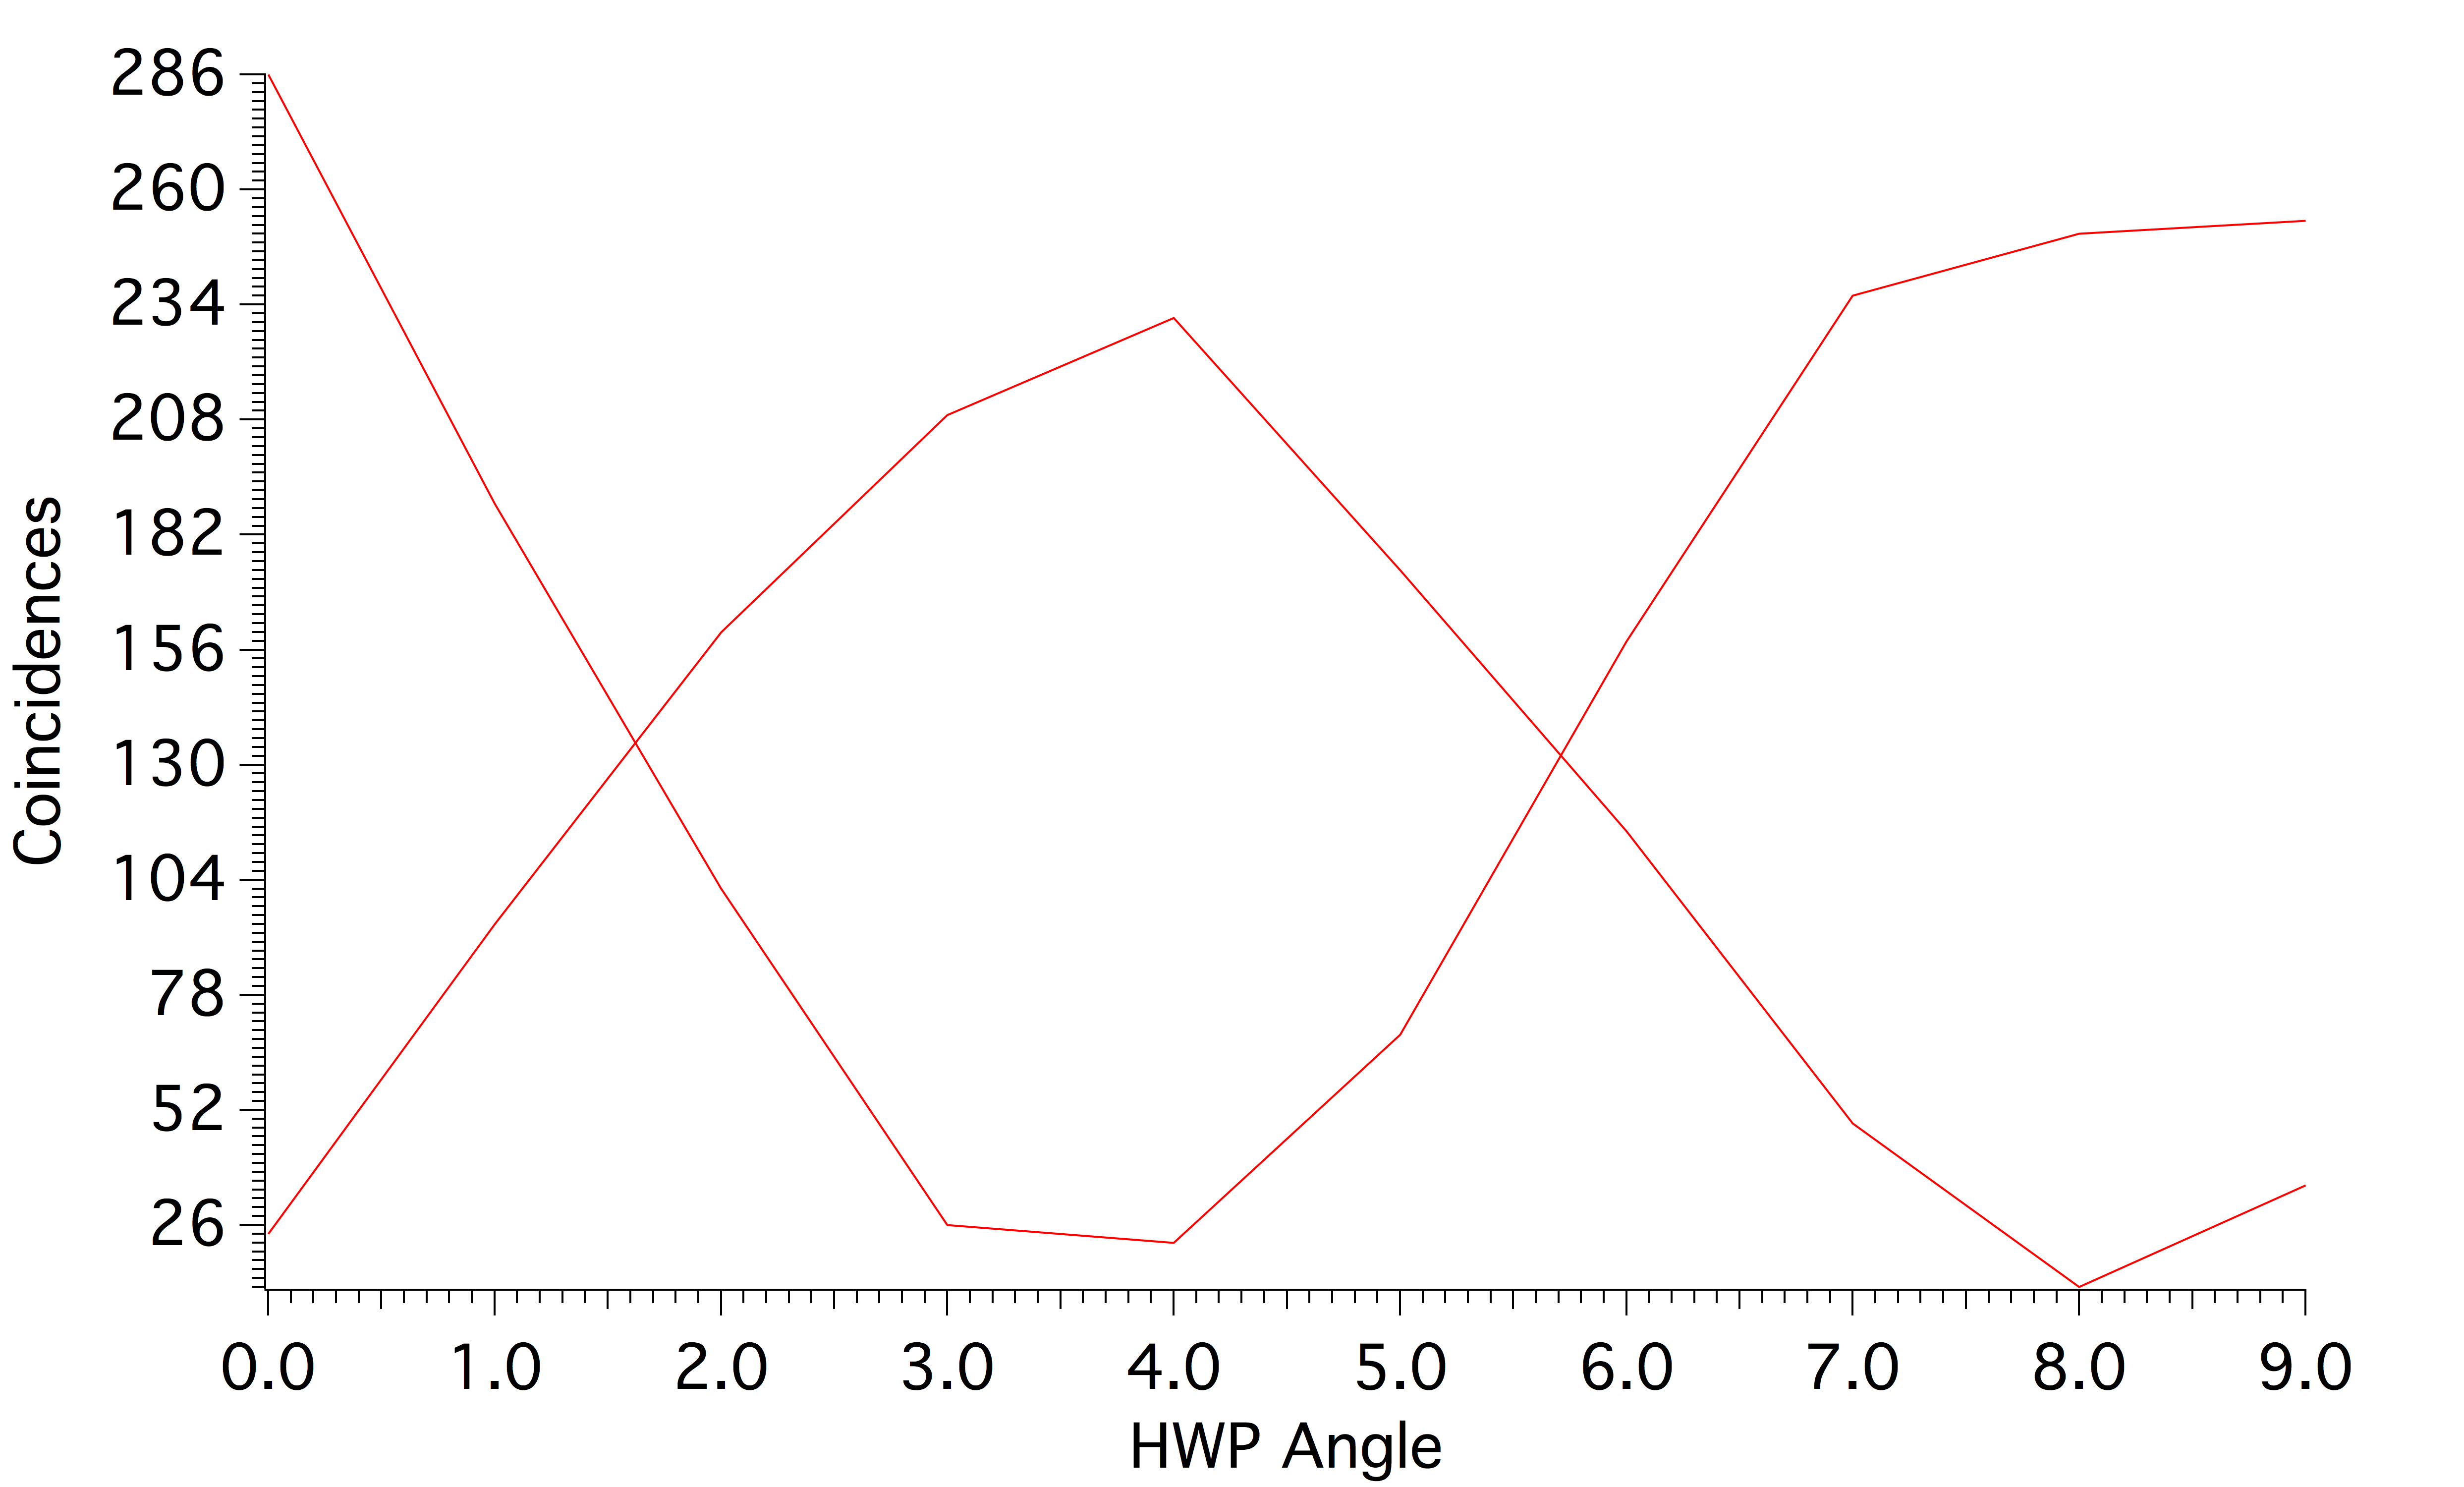
\includegraphics[width=0.9\textwidth]{equalize}
  \caption{Coincidences are equalized for (0,0) and (90,90) with HWP=16 and HWP=57. This corresponds to the HWP at $45^{\circ}$ relative to the BBO crystals' optic axes and equalizes the probability of photons downconverting in the first or second crystal. \label{fig:equalize}}
\end{figure}

A QWP was then placed before the HWP. With polarizes set to (+45, -45), coincidences were minimized with QWP=130.5. It would have been easier to maximize (+45, +45). This adjustment amounts to setting $\phi = 0$ (in Equation \ref{eq:dc}).

Coincidences were counted for varying characteristic polarization configurations, and recorded on the computer.

\section{Results and Discussion}

\subsection{Results}

For our first collection time period and a configuration with QWP=$119^{\circ}$, HWP=$16^{\circ}$, and Time=240 seconds, we confirmed that (+45, +45) (-45, -45) and (0, 0) coincide with approximately equal probability, shown in Table \ref{tab:take1}. The (-45, +45) configuration is included, but still contains a relatively large number of counts, which was further refined for our second collection period.

\begin{table}[!h]
  \centering
  \begin{tabular}{ c c }
    Polarizer Angles & Coincidences \\ \hline
    (0, 0) & 161 $\pm$ 13 \\
    (+45, +45) & 179 $\pm$ 13\\
    (-45, -45) & 181 $\pm$ 13 \\
    (-45, +45) & 22 $\pm$ 5
  \end{tabular}
  \caption{Counts with QWP=$119^{\circ}$, HWP=$16^{\circ}$, and Time=240 seconds. \label{tab:take1}}
\end{table}

During our second collection period, we minimized (+45, -45) and (-45, +45) with QWP=130.5 to coincidence levels on the same order of magnitude as (0, 90), shown in Table \ref{tab:take2},which is a good measure of 0\% probability, because it should be 0\% according to both models. Non-zero counts are due to imperfections in the polarizers and alignment of the crystals.

\begin{table}[!h]
  \centering
  \begin{tabular}{ c c }
    Polarizer Angles & Coincidences \\ \hline
    (0, 0) & 108 106 98 $\pm$ 10 \\
    (+45, -45) & 8 7 $\pm$ 3 \\
    (-45, +45) & 4 4 3 4 5 $\pm$ 2\\
    (0, 90) & 6 5 $\pm$ 2
  \end{tabular}
  \caption{Counts with QWP=130.5 HWP=16 Time=120 seconds. \label{tab:take2}}
\end{table}

These results definitively invalidate the classical model and validate the quantum model given by Equation \ref{eq:quantum} for the polarizer configurations investigated.

\section{Conclusion}

Classical and quantum coincidence models were presented for pairs of polarization correlated photons. The results of the performed experiment invalidate the classical model.

In a next experiment, coincidences for range of angle configurations should be plotted and fit to Equation \ref{eq:quantum} in order provide complete validatation of the quantum mechanical model, rather than the partial validation demonstrated here.

\begin{thebibliography}{9}
  \bibitem{einstein}
    Einstein, A; Podolsky, B; Rosen, N (1935). 
    \emph{Can Quantum-Mechanical Description of Physical Reality be Considered Complete?}
    Physical Review 47 (10): 777.
  \bibitem{bell}
    Bell, J. S. (1964). 
    \emph{On the Einstein Podolsky Rosen Paradox.} 
    Physics 1 (3): 195.
  \bibitem{bell2}
    Bell, J.S. (1966). 
    \emph{On the problem of hidden variables in quantum mechanics}. 
    Reviews of Modern Physics (38): 447.
  \bibitem{aspect}
    Aspect, A; Dalibard, J; Roger, G (1981).
    \emph{Experimental Tests of Realistic Local Theories via Bell's Theorem}.
    Phys. Rev. Lett. (47) 460.
  \bibitem{rovelli}
    Smerlak, M; Rovelli, C (2007).
    \emph{Relational EPR.}
    Found. Phys. (37): 427.
  \bibitem{dehlinger}
    Dehlinger, D; Mitchell, M.W. (2002).
    \emph{Entangled photons, nonlocality and Bell inequalities in the undergraduate laboratory}.
    Am. J. Phys. (70): 903.

\end{thebibliography}

\end{document}